\documentclass[../main.tex]{subfiles}

\graphicspath{{\subfix{../figures/}}}

\begin{document}

\gls{cryoem} is an image acquisition technique that uses \glspl{tem} to examine a frozen sample. Unlike traditional optical microscopes, \glspl{tem} use a electron beam instead of light, which allows them to capture images at much higher resolution. As a consequence, it has become a very popular technique for collecting images of biological molecules, such as proteins\cite{chemistry_world_cryoem}.

However, \glspl{tem} require very specific conditions in order to work, such as a near perfect vacuum and high-energy electrons. Therefore they are unsuitable for biological samples, as these are too fragile to endure in such conditions. Here is where the cryogenic part comes into place. In order to retain the sample intact and in place, a thin film of ice is used. The sample is cooled down very rapidly, so that the water has no time to form a crystal lattice, avoiding the diffraction of the electron beam. This technique was awarded with the 2017 Nobel Prize in Chemistry\cite{chemistry_world_cryoem}.

\begin{figure}[h]
    \centering
    \begin{subfigure}[b]{0.3\textwidth}
         \centering
         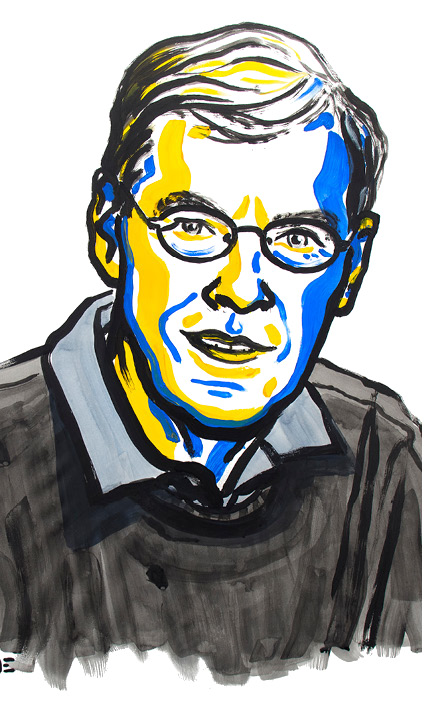
\includegraphics[width=\textwidth]{nobel2017/Richard Henderson}
         \caption{Richard Henderson}
         \label{fig:1:nobel2017:richard}
    \end{subfigure}
    \hfill
    \begin{subfigure}[b]{0.3\textwidth}
         \centering
         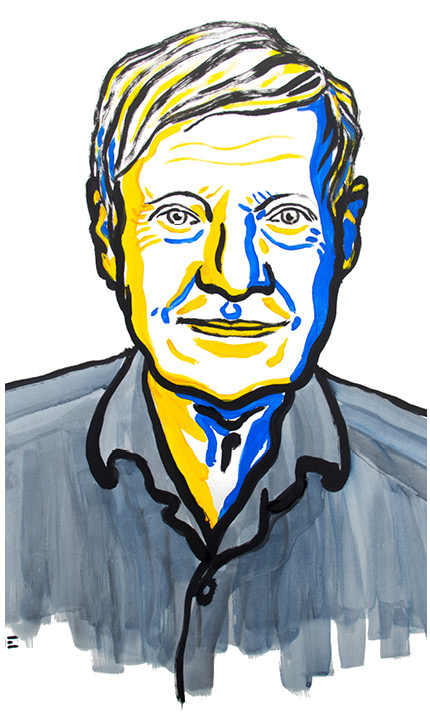
\includegraphics[width=\textwidth]{nobel2017/Joachim Frank}
         \caption{Joachim Frank}
         \label{fig:1:nobel2017:joachim}
    \end{subfigure}
    \hfill
    \begin{subfigure}[b]{0.3\textwidth}
         \centering
         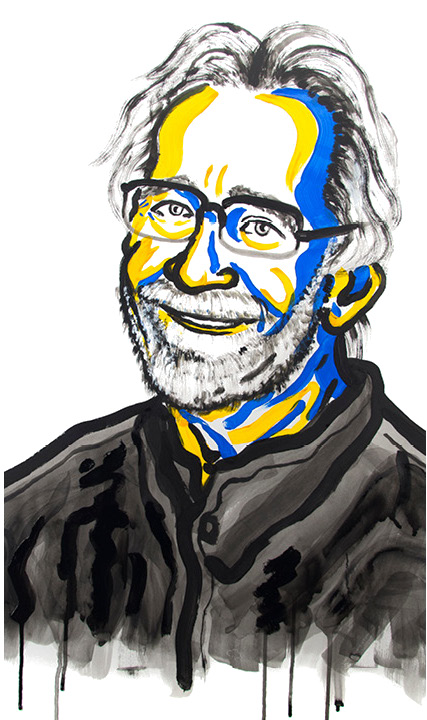
\includegraphics[width=\textwidth]{nobel2017/Jacques Dubochet}
         \caption{Jacques Dubochet}
         \label{fig:1:nobel2017:jaques}
    \end{subfigure}\\
    Images obtained from: \cite{science_nobel}
    \caption{2017 Nobel Prize in Chemistry}
    \label{fig:1:nobel2017}
\end{figure}

Usually, the sample is prepared on a copper or gold grid, which may hold thousands of specimens under study, each of them with a random orientation. Each of these specimens is known as ``particle''. Assuming that all particles belong to the same structure, their 2D projections can be used to mathematically infer the 3D structure of the specimen\cite{cryoem101}. \Gls{spa} is a family of image acquisition and processing techniques that enables such a task.

At the beginning of the \gls{spa} image processing pipeline, a large quantity of noisy data is provided, from which little to no parameters are known. Therefore, all of the parameters needed for reconstruction must be estimated from the data. The projection direction of each of the particles is among the unknowns. The process of deducing their orientation is known as particle alignment.

This work focuses on developing a fast \gls{gpu} accelerated computer program to align particles. The key innovation of this project is the usage of state-of-the-art vector search databases.

\section{Structure of the document}
TO BE COMPLETED

\end{document}
 